\documentclass[10pt]{article}
\usepackage[margin=0.8in]{geometry}
\usepackage{booktabs,graphicx,amsmath,xcolor,enumitem}
\usepackage[hidelinks]{hyperref}
\usepackage{microtype}
\usepackage[font=small,labelfont=bf]{caption}
\setlist{nosep,leftmargin=*}
\setlength{\parskip}{3pt}
\newcommand{\todo}[1]{\textcolor{red}{[#1]}}

\title{\textbf{Profile-Driven Device Placement for a RAG Pipeline}\\[2pt]
\large CSE 291A Option 2 --- Phase 1: Measurement and Profiling}
\author{Ting-Yu Yu, Cheng-Yang Wu, Jonas Tsai, Vincent Chen}
\date{November 2, 2026}

\begin{document}
\maketitle

\begin{abstract}
We profile a three-stage retrieval-augmented QA pipeline (embedding, reranking, LLM generation) on the CPU,
integrated GPU (iGPU) and NPU of an ASUS NUC 16 Pro (Intel Core Ultra 7 356H) with OpenVINO 2026.4.1.
All three stages run on all three devices with no silent fallback, which we verify both from the runtime
(\texttt{EXECUTION\_DEVICES}) and from kernel-level activity counters. With one request at a time, the iGPU is
the fastest device for every stage, and the choice of the LLM device dominates end-to-end latency
(437\,ms all-iGPU vs.\ 815\,ms with the LLM on the NPU and 1.9\,s on the CPU). The NPU becomes useful only when
stages overlap: moving the reranker to the NPU raises throughput from 2.38 to 2.50\,q/s and lowers tail
latency near saturation, at a small quality cost (recall@3 0.87$\to$0.83), because the NPU produces
slightly different reranker scores. Overlapped stages slow each other through shared DRAM, not through the
Python GIL. NPU behaviour is shaped by static shapes: compile time grows to minutes for large shapes, and the
LLM's first-token latency depends on the compiled maximum prompt length rather than on the actual prompt.
\end{abstract}

\section{Setup}

\textbf{Pipeline.} \textit{Query $\to$ S1 embed $\to$ vector search $\to$ S2 rerank $\to$ S3 generate.}
S1 is bge-small-en-v1.5 (FP16, static shape $[b,64]$), S2 is bge-reranker-base (FP16, $[k,256]$, one call
scores all $k$ candidates), and S3 is Qwen2.5-1.5B-Instruct, INT4 symmetric channel-wise weights, run with the
OpenVINO GenAI \texttt{LLMPipeline}. The same IRs and shapes are used on every device, so model and precision
are matched. Search is exact cosine search over 25{,}880 passages (numpy, CPU, $\approx$4\,ms). The prompt
contains the top-3 reranked passages; S3 generates up to 32 tokens (greedy).

\textbf{Data.} The corpus contains real Wikipedia paragraphs: every SQuAD v1.1 paragraph plus the distractor
paragraphs of 500 sampled HotpotQA questions, so every gold passage is in the corpus. Development questions:
500 sampled SQuAD v1.1 dev questions (end-to-end runs use the first 100). HotpotQA (500) is held out for
Phase~2. The LLM stage sweeps use \emph{length-controlled} prompts made of corpus text cut to exactly
256/1k/4k tokens plus a summarization instruction, with a different text per repetition, and fixed output
length (\texttt{ignore\_eos}). Real RAG prompts are 213--1{,}888 tokens (median 555 at top-3).

\textbf{Machine.} 16 cores (no SMT, AVX2/AVX-VNNI, no AVX-512/AMX), Intel Arc iGPU (\texttt{xe} driver),
Intel NPU (\texttt{intel\_vpu}, driver 1.33), 96\,GB DDR5 \emph{shared by all three devices}, Linux 7.0.
The machine is shared with other projects; we record the load average with every row (1.5--7 during our runs).

\section{Methodology}

Our harness (\texttt{scripts/harness.py}) has four modes.
(1) \textbf{Stage sweeps} measure one stage in isolation, one factor at a time: S1 batch (1/8/32 queries),
S2 candidate count (10/20/50/100, real candidates retrieved for real questions), S3 prompt length
(256/1k/4k) and output length (32/128/256). Each configuration has a separate model load, one recorded first
run (``cold run''), and 3--10 warm repetitions; we report warm medians.
(2) \textbf{End-to-end} runs process 100 dev questions under a fixed stage-to-device mapping, either
sequentially or with overlap (a front worker runs S1+search+S2 for query $i{+}1$ while a back worker runs S3 for
query $i$), and record per-stage times, EM/F1 and retrieval recall. Runs are repeated in interleaved rounds.
(3) \textbf{Load} runs drive the same two-worker pipeline with closed-loop clients (1/2/4) or open-loop Poisson
arrivals (0.5--3\,q/s); response time is measured from arrival to completion.
(4) \textbf{Contention} runs measure S3 decode while an S2 aggressor loops on another device, either in a
thread of the same process or in a separate process.

\textbf{Instrumentation} (all without root):
\begin{itemize}
  \item \emph{Placement}: \texttt{EXECUTION\_DEVICES} for S1/S2; for all stages, per-process DRM fdinfo
        (\texttt{drm-cycles-ccs}, iGPU compute-engine cycles) and the global NPU busy counter
        (\texttt{npu\_busy\_time\_us}), sampled around each measured call.
  \item \emph{Memory}: a 20\,ms sampler records peaks of process RSS, system-used memory, iGPU GTT memory
        (\texttt{drm-resident-gtt}) and NPU memory (\texttt{drm-total-}\allowbreak\texttt{memory}); model footprint = load peak $-$ baseline.
  \item \emph{Transfer}: S1/S2 calls are split into tokenize / set input / infer / get output, and infer is
        repeated with zero-copy device-context input tensors; the difference estimates the plugin input copy.
        For S3 we use GenAI's tokenize/inference/detokenize durations. End-to-end runs log the bytes handed between stages.
  \item \emph{Cold start}: \texttt{NPU\_BYPASS\_UMD\_CACHING=YES} bypasses the NPU driver's compile cache and
        \texttt{NEO\_CACHE\_PERSISTENT=0} disables the iGPU kernel cache; 3 repetitions.
\end{itemize}
\textbf{Energy was not measured.} RAPL counters are root-only on this machine and we have no other reliable
instrumentation, so we make no energy claims at any level (accelerator, package or machine).

\section{Support matrix and actual placement}

\begin{table}[h]
\centering\small
\caption{Support matrix. Load = model load + compile time with a warm compile cache / true cold. ``Busy'' is
the median share of the call's latency during which the NPU busy counter advanced; iGPU cycles were zero on
every non-iGPU run and NPU busy was zero on every non-NPU run.}
\label{tab:support}
\begin{tabular}{llllll}
\toprule
Stage & Device & Runs & Fallback & Activity evidence & Load warm / cold (s) \\
\midrule
S1 embed  & CPU & yes & none & no iGPU/NPU activity & 0.39 / 0.39 \\
          & iGPU & yes & none & $8.8\times10^4$ cycles/call & 0.44 / 1.0 \\
          & NPU & yes & none & NPU busy 92\% & 0.07 / 1.0 \\
S2 rerank & CPU & yes & none & no iGPU/NPU activity & 3.3 / 3.3 \\
          & iGPU & yes & none & $3.6\times10^6$ cycles/call & 3.1 / 3.8 \\
          & NPU & yes$^{a}$ & none & NPU busy 91\% & 0.12 / 68 \\
S3 LLM    & CPU & yes & none$^{b}$ & no iGPU/NPU activity & 0.67 / 0.67 \\
          & iGPU & yes & none$^{b}$ & $3.7\times10^7$ cycles/call & 1.6 / 3.0 \\
          & NPU & yes$^{c}$ & none$^{b}$ & NPU busy 95\% & 4.9 / 10.8 \\
\bottomrule
\end{tabular}\\[2pt]
\raggedright\footnotesize
$^{a}$Static shapes only; 50 candidates take 241\,s to compile, 100 candidates 21\,min and then run at 14.2\,s per call
(iGPU: 0.52\,s). Scores differ slightly from CPU/iGPU (Sec.~\ref{sec:quality}).
$^{b}$\texttt{LLMPipeline} does not report \texttt{EXECUTION\_DEVICES}; placement is established from activity counters only.
$^{c}$Requires symmetric INT4 weights: the asymmetric INT8 export compiles on the NPU but generates garbage.
The NPU LLM must share no process with another NPU model since 2026-11 (Sec.~\ref{sec:neg}). Load shown for a
1{,}152-token maximum prompt.
\end{table}

All nine stage--device pairs run, and the activity counters agree with the requested device in every case
(Table~\ref{tab:support}): there is no silent CPU fallback, including for the LLM, where the runtime itself does
not report placement. The NPU, however, is the least flexible device. It requires static input shapes,
including a maximum prompt length for the LLM, which is fixed at compile time. Compile cost grows quickly with
shape size. The OpenVINO NPU compile cache hides this after the first load: the reranker's load time is 0.12\,s
with a warm cache but 68\,s cold. The iGPU also compiles kernels, but cold loads cost only 0.5--1.4\,s more.

\section{Per-stage profiles}

\begin{figure}[t]
\centering
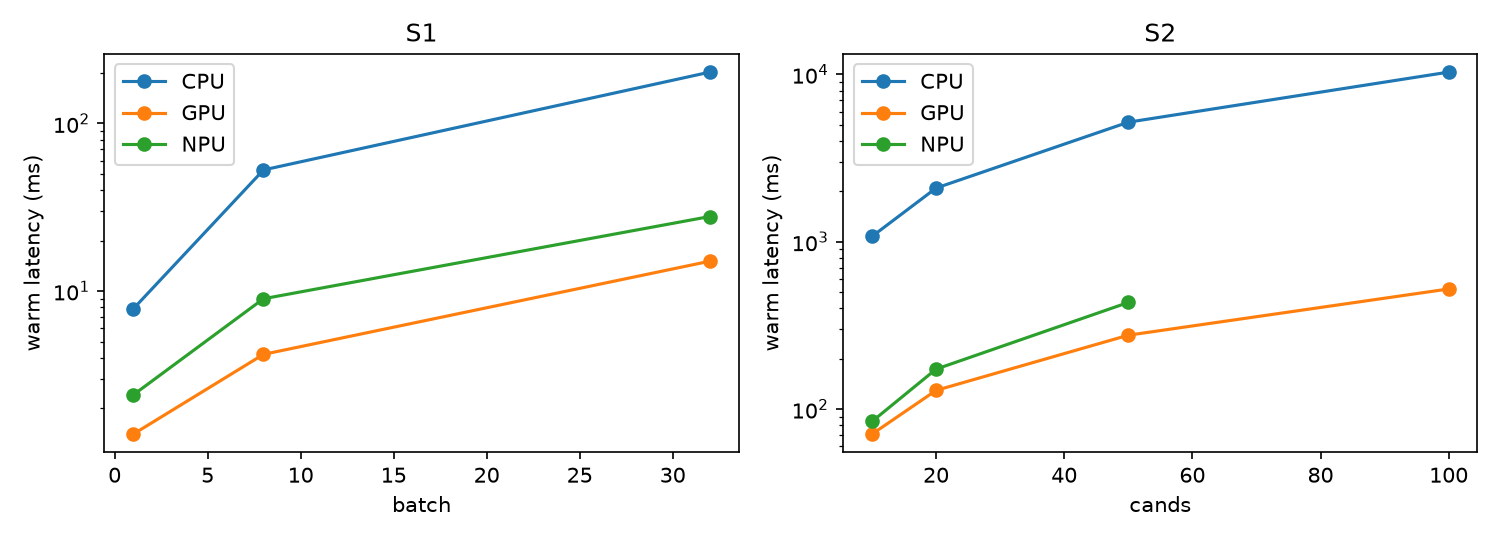
\includegraphics[width=0.8\linewidth]{fig/fig_stage_S1_S2.png}\\[2pt]
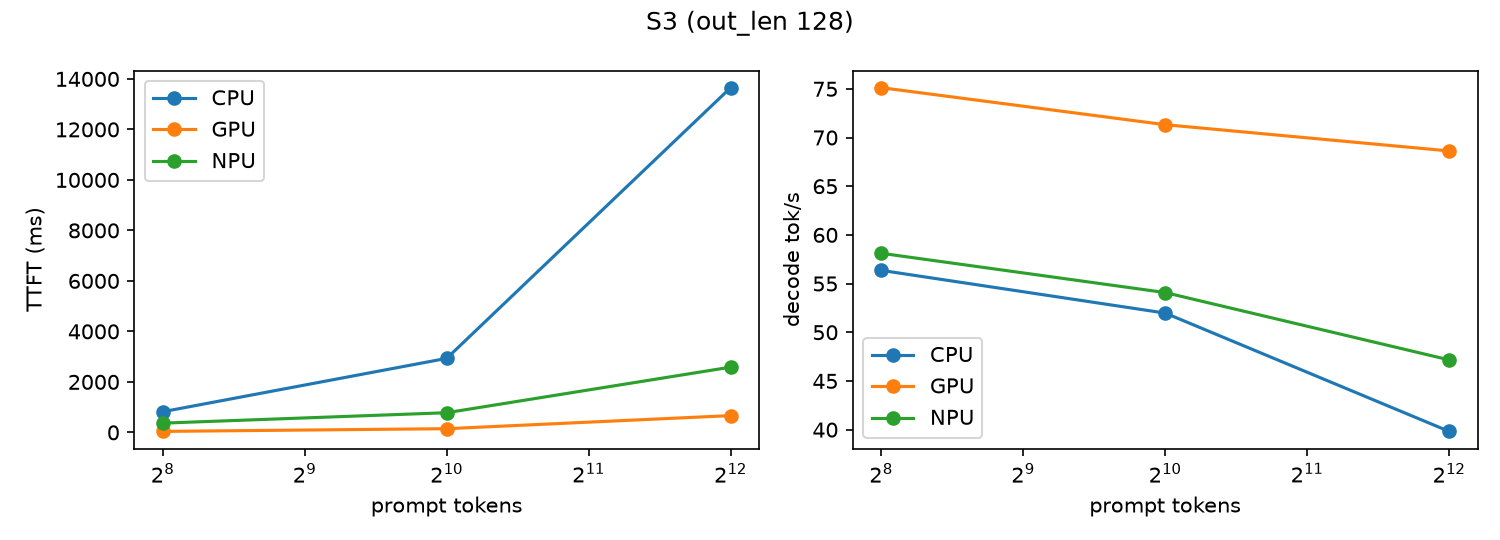
\includegraphics[width=0.8\linewidth]{fig/fig_stage_S3.png}
\caption{Warm per-stage latency (``GPU'' = iGPU). Top: S1 vs.\ batch size (queries), S2 vs.\ candidate count (log scale;
NPU at 100 candidates, 14.2\,s, omitted). Bottom: S3 time to first token (TTFT) and decode rate vs.\
prompt length, output 128 tokens; the NPU points use one pipeline compiled for a 4{,}224-token maximum prompt.}
\label{fig:stages}
\end{figure}

\begin{table}[t]
\centering\small
\caption{Warm medians (ms). S3: TTFT / time per output token (TPOT). NPU S3 TTFT is given for a pipeline compiled
for the prompt length (max.\ prompt 384/1152/4224) and, in parentheses, for one compiled for 4{,}224 tokens.}
\label{tab:stages}
\begin{tabular}{lrrr@{\hspace{2.2em}}lrrr}
\toprule
S1 batch & CPU & iGPU & NPU & S2 cands & CPU & iGPU & NPU \\
\midrule
1  & 7.8 & 1.4 & 2.4 & 10 & 1{,}076 & 71 & 84 \\
8  & 52.8 & 4.2 & 9.0 & 20 & 2{,}092 & 129 & 173 \\
32 & 202 & 15.1 & 27.9 & 50 & 5{,}180 & 276 & 434 \\
   &     &      &      & 100 & 10{,}319 & 522 & 14{,}200 \\
\midrule
S3 prompt & \multicolumn{3}{c}{TTFT: CPU / iGPU / NPU} & & \multicolumn{3}{c}{TPOT: CPU / iGPU / NPU} \\
\midrule
256  & 819 & 39 & 100 (366) & & 17.7 & 13.3 & 17.4 \\
1k   & 2{,}932 & 146 & 771 (779) & & 19.2 & 14.0 & 18.6 \\
4k   & 13{,}652 & 665 & 2{,}583 & & 25.1 & 14.6 & 21.2 \\
\bottomrule
\end{tabular}
\end{table}

\textbf{S1 (embedding)} is negligible in the pipeline: 1.4--7.8\,ms per query at batch 1. The iGPU is fastest
at every batch size and the CPU scales worst (202\,ms at batch 32). At batch 1 all three devices are dominated by fixed
overhead: 54--65\% of the 64-token input is padding, yet shortening it barely changes latency.

\textbf{S2 (rerank)} is the most expensive retrieval stage and is linear in candidate count on CPU and iGPU. The iGPU
is fastest at every size (71--522\,ms). The NPU is 1.2--1.6$\times$ slower up to 50 candidates and then breaks
down at 100 (14.2\,s, 27$\times$ the iGPU). The CPU is 15--20$\times$ slower than the iGPU. S2 cost is also linear in
sequence length (20 candidates at seq.\ 128/192/256: iGPU 48/73/99\,ms), and 30\% of the computed tokens are padding
while 12.6\% of real candidate pairs are truncated at 256 tokens.

\textbf{S3 (generation).} The iGPU is fastest in both phases: its prefill is about 20$\times$ faster than the CPU's and 2.5--4$\times$ faster than the NPU's and
its decode runs at 69--75\,tok/s. Decode is memory-bandwidth bound, so the gap is smaller there: the NPU (47--58\,tok/s)
and CPU (40--56\,tok/s) are close at short prompts, while the CPU slows most with context. Output length only
scales total time (TPOT is constant across 32/128/256 tokens on the iGPU). The NPU's TTFT depends on the compiled
maximum prompt length, not on the actual prompt: a 256-token prompt takes 100\,ms with a 384-token pipeline but
366\,ms with a 4{,}224-token pipeline, because the NPU prefills the full static shape.

\section{Initialization, memory and data movement}

\textbf{Initialization.} Table~\ref{tab:support} separates warm-cache and true cold loads. The first inference
after loading costs an extra 8--12\,ms on the iGPU (S1) and up to 2$\times$ the warm latency on the NPU (S2: 199
vs.\ 84\,ms at 10 candidates). The NPU's cold costs grow with shape: the NPU LLM takes 2.0/4.9/6.2\,s to load
(warm cache) for maximum prompts of 384/1{,}152/4{,}224 tokens.

\textbf{Memory} (model footprint = load peak minus baseline). S1: 32--130\,MB of iGPU memory or 67--91\,MB of NPU
memory. S2: 0.6--1.3\,GB on the iGPU (grows with candidates; 2.0\,GB peak at 100) and 0.63/0.73/0.98\,GB on the NPU
at 10/20/50 candidates; an uncached NPU compile additionally needs 1.7--3.2\,GB of host RAM. S3: 1.0\,GB on the iGPU,
1.35/1.89/2.03\,GB on the NPU for maximum prompts of 384/1{,}152/4{,}224. An entire end-to-end process uses 1.7--2.4\,GB of
RSS. Memory is not a constraint for this pipeline on a 96\,GB machine, but the NPU LLM's footprint grows with its
static prompt shape.

\textbf{Data movement.} The three devices share DRAM, so ``transfer'' is a host-side copy, not a bus crossing. The
payload between stages is small (per query: 1.5\,KB query vector, 14.6\,KB of candidate text, 2.4\,KB prompt).
The iGPU plugin's input copy costs 3--13\,ms per S2 call ($\le$10\% of S2); on the NPU and for S1 it is below
0.4\,ms. Host-side tokenization is the larger cost: 8--35\,ms per S2 call (10--15\% of iGPU S2), while S3
tokenization and detokenization take under 2\,ms.

\section{End-to-end results}

\begin{table}[t]
\centering\small
\caption{End-to-end, 100 SQuAD dev questions, top-3 passages, warm. Sequential = one query at a time;
overlap = S1+S2 of query $i{+}1$ run during S3 of query $i$. Rows with overlap numbers: 3 rounds, std of q/s $\le 0.01$; others: 1 round.
Representative mappings of all 27 measured; mappings that differ only in S1 are within 3\%.}
\label{tab:e2e}
\begin{tabular}{lrrrrrrr}
\toprule
Mapping (S1/S2/S3) & median ms & p90 ms & S2 ms & S3 ms & q/s seq. & q/s overlap & recall@3 / F1 \\
\midrule
iGPU/iGPU/iGPU & 437 & 621 & 118 & 316 & 2.23 & 2.38 & 0.87 / 0.36 \\
NPU/NPU/iGPU   & 559 & 755 & 231 & 321 & 1.74 & \textbf{2.50} & 0.83 / 0.34 \\
NPU/iGPU/iGPU  & 437 & 627 & 117 & 317 & 2.21 & 2.38 & 0.87 / 0.36 \\
NPU/NPU/NPU    & 816 & 1{,}089 & 169 & 642 & 1.21 & -- & 0.83 / 0.33 \\
iGPU/iGPU/NPU  & 842 & 1{,}095 & 121 & 709 & 1.20 & -- & 0.87 / 0.38 \\
iGPU/iGPU/CPU  & 1{,}866 & 2{,}445 & 126 & 1{,}731 & 0.52 & -- & 0.87 / 0.34 \\
NPU/CPU/iGPU   & 2{,}435 & 2{,}621 & 2{,}092 & 332 & 0.41 & 0.47 & 0.87 / 0.36 \\
CPU/CPU/CPU    & 3{,}860 & 4{,}392 & 2{,}097 & 1{,}729 & 0.26 & -- & 0.87 / 0.34 \\
\bottomrule
\end{tabular}
\end{table}

\textbf{All 27 mappings} were measured sequentially (Table~\ref{tab:e2e} lists representatives). Latency is set by the
S3 device first and the S2 device second: S3 on the iGPU gives 437--573\,ms, on the NPU 815--845\,ms and on the CPU
1.9--2.0\,s, and S2 on the CPU adds about 2\,s. S1 placement does not matter (within 3\%). For a single user issuing
one query at a time, \textbf{the best single device (all-iGPU) is also the best mapping}: no heterogeneous mapping beats it.

\textbf{Overlap.} When query $i{+}1$'s retrieval overlaps query $i$'s generation, all-iGPU gains only 7\% (2.23$\to$2.38\,q/s)
because both stages compete for the same device. Putting S2 on the NPU lets the stages run on different devices:
throughput rises 44\% over its own sequential run (1.74$\to$2.50\,q/s) and is the highest of all mappings, 5\% above
all-iGPU overlap. S3 on the iGPU slows from 316 to $\approx$385\,ms in that configuration (Sec.~\ref{sec:causes}).

\begin{figure}[t]
\centering
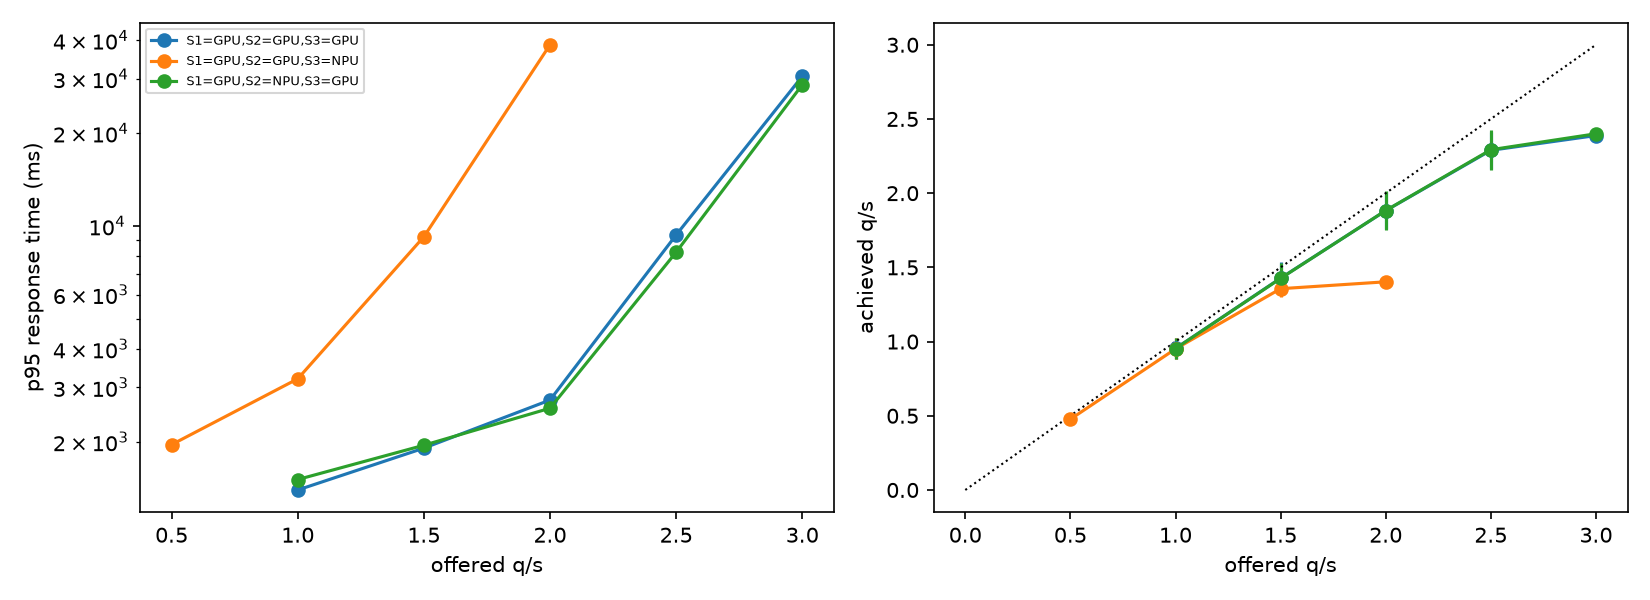
\includegraphics[width=0.78\linewidth]{fig/fig_load.png}
\caption{Open-loop Poisson load, 3 rounds of 150--300 queries per point. Left: p95 response time (log scale);
right: achieved vs.\ offered rate. All mappings use S1 on the iGPU (``GPU'').}
\label{fig:load}
\end{figure}

\textbf{Load.} Under Poisson arrivals (Fig.~\ref{fig:load}), all-iGPU and S2-on-NPU both saturate at
$\approx$2.4\,q/s, while S3 on the NPU saturates at 1.4\,q/s (1.2\,q/s if S2 is also on the NPU). Below saturation
all-iGPU has lower latency (p50 at 1\,q/s: 606 vs.\ 732\,ms); near and past saturation S2-on-NPU has lower latency
(p50 at 2.5\,q/s: 2.9 vs.\ 3.2\,s; at 3\,q/s: 9.9 vs.\ 11.7\,s), consistent with an independent 2-round run (p50 at
2.3\,q/s: 1.71 vs.\ 1.86\,s). The best mapping therefore \emph{changes with load}, which is the main input for the
Phase~2 placement policy. Above capacity, queues grow for the whole run, so those latencies depend on the run length.

\textbf{More context.} Giving S3 more passages raises recall but lowers answer quality for this 1.5B model
(all-iGPU, top-1/3/8: recall 0.74/0.87/0.90, F1 0.40/0.36/0.25) and increases S3 time (330 vs.\ 644\,ms at top-1 vs.\ top-8).

\section{Causes of device differences}
\label{sec:causes}

\textbf{Shared-memory contention, not the GIL.} To explain why S3 slows when it overlaps S2, we measured iGPU
decode (1k prompt, 3 rounds) under different aggressors:
\begin{center}\small
\begin{tabular}{llr}
\toprule
S3 device & Aggressor & TPOT (ms) \\
\midrule
iGPU & none & 14.0 \\
iGPU & S2 on NPU, same process (thread) & 22.1 \\
iGPU & S2 on NPU, separate process & 22.1 \\
iGPU & tokenization only, thread (holds the GIL, no accelerator work) & 14.2 \\
iGPU & S2 on CPU, separate process & 15.2 \\
NPU & none / S2 on iGPU, separate process & 18.6 / 31.5 \\
\bottomrule
\end{tabular}
\end{center}
A thread and a process cause the same slowdown, and a GIL-only aggressor causes none, so the slowdown is not caused
by Python. It is largest when the iGPU and NPU run at the same time (+58\% and +70\% TPOT) and the aggressor slows
too (NPU rerank: 4.4 vs.\ 5.8 calls/s alone). Both accelerators stream weights and activations from the same DRAM,
and decode is bandwidth bound. This bounds the benefit of overlap and must be part of a placement model.

\textbf{Static shapes on the NPU} explain its LLM TTFT (prefill of the full compiled length), its compile times and
its breakdown at 100 candidates. \textbf{Padding} costs all devices equally: 30\% of S2 tokens are padding.
\textbf{Prefix caching} in GenAI makes repeated prompts look nearly free on CPU/iGPU (4k-token CPU TTFT 11\,s cold,
77\,ms on repeat) but not on the NPU; our first S3 sweep was invalid for this reason and was re-run with fresh prompts.

\label{sec:quality}
\textbf{Output quality.} S1 and S3 placement do not change retrieval, and S2 on CPU and iGPU give identical
rankings. S2 on the NPU gives slightly different scores and changes the top-3 order: recall@3 drops from 0.87 to
0.82--0.83 and F1 by 0.01--0.06. S3 on the CPU or NPU gives F1 0.32--0.38 vs.\ 0.36 on the iGPU (different
kernels, same INT4 weights; 100 questions). Placement is therefore not quality-neutral and quality must be reported
next to latency.

\section{Negative results and limitations}
\label{sec:neg}
\begin{itemize}
  \item For sequential single-user queries, \textbf{no heterogeneous mapping beats all-iGPU}; the NPU is never the
        fastest device for an individual stage. Its benefit appears only with overlapped requests.
  \item The NPU reranker is unusable at 100 candidates (21-min compile, 14.2\,s per call).
  \item \textbf{Two NPU models in one process now fail}: since 2026-11, loading the NPU LLM together with another NPU
        model in the same process invalidates the first model (Level Zero null-handle error at first inference),
        although the same all-NPU configuration ran on 2026-10-27 and the software versions are unchanged. We run S3 in
        a separate process for those mappings; the extra IPC is 0.45\,ms per query, and an iGPU/iGPU/NPU control gives
        842 vs.\ 845\,ms in-process. The all-NPU result is 816\,ms in both setups.
  \item Energy was not measured (no reliable non-root instrumentation).
  \item The machine is shared: the load average was 1.5--7 during runs. Round-to-round throughput std is
        $\le$0.01\,q/s, but absolute CPU numbers may be slightly pessimistic.
  \item The LLM stage sweeps use length-controlled prompts; real RAG prompts are 213--1{,}888 tokens.
\end{itemize}

\section{Device preference and Phase 2 inputs}

\begin{table}[h]
\centering\small
\caption{Which device under which condition (Phase 1 conclusion).}
\label{tab:prefer}
\begin{tabular}{p{0.13\linewidth}p{0.37\linewidth}p{0.42\linewidth}}
\toprule
Stage & Preferred device & Conditions / exceptions \\
\midrule
S1 embed & iGPU, but any device works & $<$10\,ms per query on every device; avoid CPU for batches ($\ge$8). \\
S2 rerank & iGPU alone; NPU when overlapping S3 & NPU only $\le$50 candidates with a precompiled shape, and it costs $\approx$4 points of recall@3; never CPU. \\
S3 LLM & iGPU & NPU $\approx$1.9$\times$ slower e2e, with TTFT tied to its compiled max prompt; CPU only as a fallback. \\
Pipeline & all-iGPU at low load; S2 on NPU at high load & Crossover near 2--2.5\,q/s; GPU+NPU overlap costs up to +58\% S3 TPOT. \\
\bottomrule
\end{tabular}
\end{table}

For Phase~2, the profiles above give the inputs for a lookup-table placement policy: per-stage latency as a
function of candidate count and prompt length, model load and compile cost (including NPU static shapes), memory
footprint, and a contention penalty for stages that overlap on the iGPU and NPU. We will evaluate it against fixed
mappings and the best static configuration on held-out HotpotQA, mixed prompt lengths and varying load.

\vspace{4pt}\noindent\footnotesize\textbf{Artifacts.} Code: \texttt{scripts/} (\texttt{harness.py}, \texttt{rag\_common.py},
\texttt{run\_phase1*.sh}, \texttt{analyze\_phase1*.py}). Each run folder in \texttt{runs/} holds raw JSONL results, a
code snapshot, the git revision, \texttt{pip freeze}, the environment at start and end, and its analysis:
\texttt{2026-10-27\_155708} (Phase 1 sweeps and 9 mappings with overlap),
\texttt{2026-10-27\_182944} (S3 with fresh prompts),
\texttt{2026-10-28\_212940} (memory, placement, transfer, cold start, concurrency, contention),
\texttt{2026-11-01\_170003} (all remaining mappings, prompt size, load sweep),
\texttt{2026-11-02\_080003} (NPU mappings with S3 in its own process).
\end{document}
